% Introduction

\chapter*{Introduction}
\label{intro} % For referencing the chapter elsewhere, use \ref{Chapter1} 

\lhead{Introduction \emph{Presenting the canvas, etc}} % This is for the header on each page - perhaps a shortened title

%----------------------------------------------------------------------------------------

\section{What is a Physics Simulation?}

\hspace{.5cm} The purpose of this thesis is to present a series of physics simulations, each modeling a specific problem of physics as realistically as possible.  These simulations differ from \textit{animations}, which are predictable representations that always display the same visual.  Animations are analagous to a movie script: they always end in the same way.  Simulations, on the other hand, need to adapt to variable conditions, and may be based partly on random processes.  This brings up the topic of \textit{dynamic} vs. \textit{static} animation.  Most of the physics simulations in this thesis will be dyamic because they present a unique viewing each time they are run, and can also involve user input which influences the outcome of the simulation.

Any simulation requires creating the illusion of motion.  Almost every form of projected motion media uses frames to accomplish this.  Researchers have shown that to make a simulation look realistic, it must be presented at a rate of around 60-100 frames per second.\textsuperscript{\cite{jsbook}}  Anything slower and the human eye will detect the ``choppiness'' of the simulation.  People can't detect anything much faster than 100 frames per second, so there is no need to project media faster than that, with the exception of slow-motion videography.  




%----------------------------------------------------------------------------------------


\section{Methods of Producing a Simulation}

The physics simulations in this thesis differ greatly from common animations.  Movies and cartoons, for example, operate by displaying a series of images similar to one another, and displaying them as many frames per second to create the illusion of motion.  My simulations, on the other hand, function by providing the \textit{information} for each frame, and then providing the data for \textit{how} the animation can be created.  These instructions are passed onto the HTML5 canvas API, which creates the visual which can be seen in the web browser.\textsuperscript{\cite{basichtml5}}  Because physics simulations contain instructions instead of a series of images, the files of code take up far less space than a movie file would, for example.  This is one primary advantage of coded simulations.  Every simulation follows a similar set of steps, which can be simplified below: 

\begin{figure}[h] 
	\centering
		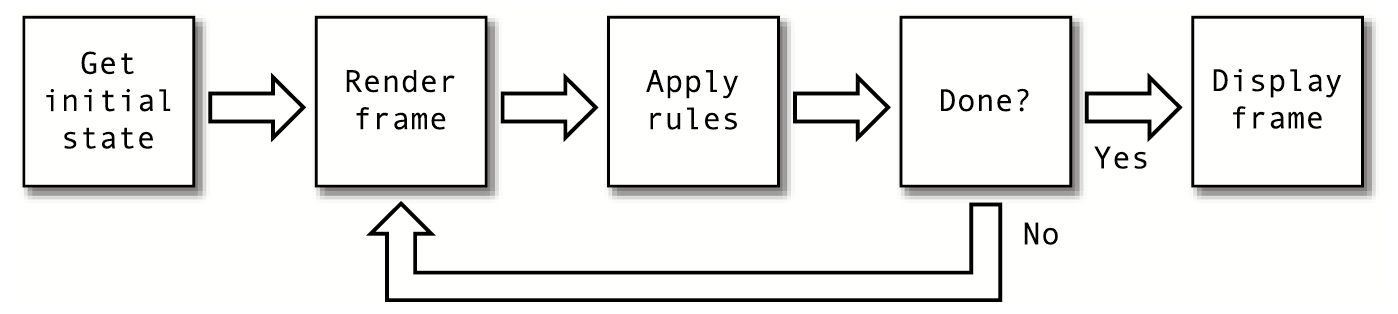
\includegraphics[width=15cm]{Figures/frames.png}

	\caption{The frames of a general simulation}
	\label{fig:frames}
\end{figure}


The canvas API gets the initial state of the simulation, which could the position of a ball, for example.  Then, the frame is \textit{rendered} by applying rules to the canvas element, and changing the initial state of the simulation.  Once the rules have been applied, and all conditions are satisfied, the frame is rendered, and then displayed on the canvas element, to be seen in the web browser.\textsuperscript{\cite{basichtml5}}  The canvas is embedded into a web page with the \textless canvas\textgreater tag, like any other HTML tag.  The positioning of objects in the canvas element is specified with a coordinate system, which uses pixels as its unit.  Figure \ref{fig:canvas} shows the orientation of the canvas, which differs from the traditional cartesian coordinate system.

\begin{figure}[h] 
	\centering
		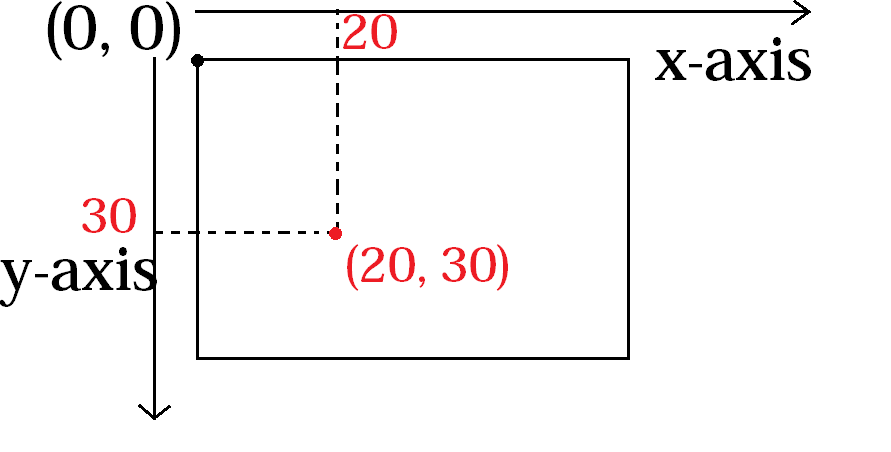
\includegraphics[width=8cm]{Figures/canvas.png}

	\caption{The canvas coordinate system.  The canvas is displayed on the screen as a white rectangle by default.  A sample point of (20,30) is shown for clarification.}
	\label{fig:canvas}
\end{figure}



To produce any realistic simulation, the steps in figure \ref{fig:frames} must be repeated multiple times per second.  In fact, these steps must be repeated 60 times per second to achieve the desired 60 frames per second outlined in the previous section.  Luckily, the canvas API is capable of running the instructions very quickly to make this simulation possible.  





%----------------------------------------------------------------------------------------





\subsection{The Code}

To program the simulations in this thesis, I chose to write the code in JavaScript (JS).  This scripting language is easy to view in any modern browser: therefore, all the simulations of this thesis can be viewed online.  JavaScript combines seamlessly with HTML5, which is why I mostly decided to use it for this thesis.  The evolution of HTML (HyperText Markup Language) has progressed from simple web documents to complex web applications.  For this thesis, every simulation utilizes the HTML5 \textless canvas\textgreater element, which has been used since around 2011.\textsuperscript{\cite{basichtml5}}  The HTML5 canvas API allows programmers to write JS code that accesses the element and runs visual displays through a web browser  The HTML needed to include a canvas can seen below:



\vspace{1cm}
\setstretch{1}
\begin{lstlisting}[breaklines=true, frame=single, numbers=left, caption= The bare bones code necessary for an HTML document to include the canvas element.  The canvas in this situation is a 500 pixel square., label=lst:basichtml]  
<!doctype html>
<html>
 <body>
  <canvas id="canvas" width="500" height="500" >  
 </body>
 <script>
  var canvas = document.getElementById('canvas');
  var context = canvas.getContext('2d');
 </script>
</html>

\end{lstlisting}
\setstretch{2}

The above code displays the most basic HTML combined with JavaScript necessary to begin any simulation.  Lines 7-8 are the only ones that actually contain JavaScript: this is the simple step necessary for the canvas API to recognize the HTML document.  These two steps are necessary for any physics simulation.  The step on line 7 initializes a JS variable and sets it equal to the canvas element on the web document object.  The second step on line 8 connects to the canvas context, which is necessary for actually sending information to be displayed.  Multiple canvases can be used, and each canvas has a separate context used for ``drawing'' to. 

All web browsers include some form of JavaScript interpreter: whenever the browser encounters a \textless script \textgreater element, it     ``passes''  the code onto the JS interpreter.\textsuperscript{\cite{jsdefinitive}}  In listing \ref{lst:basichtml}, the HTML and JS code are written in the same document for clarity.  While this is an acceptable practice, all future simulations will involve the HTML referencing to external JS documents to keep the contents separate.  The appendices in this thesis have full code files from all of the simulations.  

While this thesis can contain code excerpts, figures, and screen-shots of various simulations, it obviously can't contain the flow of images itself.  Therefore, I have put the entire thesis and its simulations on my personal website, which can be found at:  http://www.peterkrieg.com/thesis.  You can navigate by each chapter and view the simulations outlined in thesis. 




